\documentclass[english,serif,mathserif,xcolor=pdftex,dvipsnames,table]{beamer}

\usepackage[T1]{fontenc}
\usepackage[utf8]{inputenc}

\usetheme[informal]{s3it}
\usepackage{s3it}

\title[3. Sequences and loops]{%
  A Short and Incomplete Introduction to Python
}
\subtitle{\bfseries Part 3: Sequences and \texttt{for}-loops}
\author[R.~Murri]{%
  \textbf{Riccardo Murri} \texttt{<riccardo.murri@uzh.ch>}, \\
  Sergio Maffioletti \texttt{<sergio.maffioletti@uzh.ch>}
  \\
  S3IT: Services and Support for Science IT,
  \\
  University of Zurich
}
\date{January 14, 2019}


\begin{document}

% title frame
\maketitle


\part{Lists and sequences}

\begin{frame}
  \frametitle{Sequences}

  Python provides a few built-in \emph{sequence} classes:
  \begin{description}
  \item[list] \emph{mutable}, possibly heterogeneous
  \item[tuple] \emph{immutable}, possibly heterogeneous
  \item[str] \emph{immutable}, only holds characters
  \item[bytes] \emph{immutable}, only holds bytes
  \end{description}

  \+
  Additional sequence types \\ are provided by external modules:
  \begin{description}
  \item[array] \emph{mutable}, homogeneous \\ (like C/Fortran arrays,
    from~\href{http://numpy.scipy.org}{NumPy})
  \item[DataFrame] \emph{mutable}, heterogeneous \\ (like R,
    from~\href{http://pandas.pydata.org/}{Pandas})
  \end{description}

\end{frame}


\begin{frame}[fragile]
  \frametitle{List basics}
  Lists are by far the most common and used sequence type in Python.

  \+
  Lists are created and initialized by enclosing values into
  `\texttt{[}' and `\texttt{]}':
\begin{lstlisting}
>>> L = [ 'U', 'Z' ]
\end{lstlisting}

  \+
  An empty list is created by a pair of square brackets with
  nothing in between:
\begin{lstlisting}
>>> K = [ ]
\end{lstlisting}

\end{frame}

\begin{frame}[fragile]
  \frametitle{List basics, II}

  You can append and remove items from a list:
\begin{lstlisting}
>>> L = [ 'U', 'Z' ]
>>> L.append('H')
>>> print (L)
['U', 'Z', 'H']
\end{lstlisting}

  \+\pause
  You can append \textbf{any} object to a list:
\begin{lstlisting}
>>> L.append([1, 2])
>>> print(L)
['U', 'Z', 'H', [1, 2]]
\end{lstlisting}

  % % \+
  % \begin{references}
  %   \url{http://docs.python.org/tutorial/datastructures.html#more-on-lists}
  % \end{references}
\end{frame}


\begin{frame}[fragile,fragile]
  \frametitle{Sequences, II}
  You can access individual items in a sequence using the postfix
  \texttt{[]} operator.

  \+
  Sequence indices start at 0.

\begin{lstlisting}
>>> L = ['U', 'Z', 'H']
>>> print(L[0], L[1], L[2])
'U' 'Z' 'H'
>>> S = 'UZH'
>>> print(S[0], S[1], S[2])
'U' 'Z' 'H'
\end{lstlisting}
\end{frame}


\begin{frame}[fragile]
  \frametitle{Sequence length}
The \texttt{len()} function returns the number of items in any
  sequence (not just lists).
\begin{lstlisting}
>>> len(L)
3
\end{lstlisting}

  \+ Built-in functions \lstinline|sum()|, \lstinline|max()|, \lstinline|min()|
  also work on list arguments.
\end{frame}


\begin{frame}
  \begin{exercise*}[3.A]
    Write a function \texttt{avg()} that takes a list of numbers and returns
    their mean value.
  \end{exercise*}
\end{frame}


\begin{frame}[fragile]
  \frametitle{Slices}
  The notation \texttt{[$n$:$m$]} is used for accessing a \emph{slice}
  of sequence (the items at positions $n$, $n+1$, \ldots, $m-1$).

\begin{lstlisting}
>>> # list numbers from 0 to 9
>>> R = list(range(0,10))
>>> R[1:4]
[1, 2, 3]
\end{lstlisting}

  \+
  If $n$ is omitted it defaults to 0, if $m$ is omitted it defaults to
  the length of the sequence.

  \+ A \textit{slice} of a sequence is a sequence \textit{of the same
  type}.
\begin{lstlisting}
>>> S = 'zurich'
>>> S[0:4]
'zuri'
\end{lstlisting}
\end{frame}


\begin{frame}[fragile]
  \frametitle{List mutation}
  You can replace items in a \emph{mutable} sequence by assigning them
  a new value:
\begin{lstlisting}
>>> L = ['P', 'y', '2']
>>> L[2] = '3'
>>> print(L)
['P', 'y', '3']
\end{lstlisting}

\end{frame}
\begin{frame}[fragile]
  \frametitle{List mutation}

You can also replace an entire slice of a mutable sequence:
\begin{lstlisting}
>>> L[0:2] = ['1', '2']
>>> print(L)
['1', '2', '3']
\end{lstlisting}

The new slice does not need to have the same length:
\begin{lstlisting}
>>> L[2:] = range(5)
>>> print(L)
['1', '2', 0, 1, 2, 3, 4]
\end{lstlisting}
\end{frame}


\begin{frame}[fragile]
  \frametitle{Lists operators}
  You can concatenate two lists using the \texttt{+} operator:
  \begin{lstlisting}
>>> [1, 2] + [3, 4]
[1, 2, 3, 4]
  \end{lstlisting}

  \+
  You can mutate a list \emph{in place} with the \texttt{+=} operator:
  \begin{lstlisting}
>>> L = [1, 2]
>>> L += [3, 4]
>>> print(L)
[1, 2, 3, 4]
  \end{lstlisting}

\+
The \texttt{*} operator also works on lists:
  \begin{lstlisting}
>>> L = [1, 2]
>>> print(L*3)
[1, 2, 1, 2, 1, 2 ]
  \end{lstlisting}
\end{frame}


\begin{frame}[fragile]
  \frametitle{Operating on lists}

  Python provides a number of methods to modify a list~\texttt{L}:

  \begin{describe}{L.append(x)}
    Append item \texttt{x} to list \texttt{L}.
  \end{describe}

  \begin{describe}{L.insert(n, x)}
    Insert item \texttt{x} at position \texttt{n} of list \texttt{L};
    other items are ``shited to the right'' to make place.
  \end{describe}

  \begin{describe}{L.pop(n)}
    Remove item at position \texttt{n} from list \texttt{L}.
  \end{describe}

  \begin{describe}{L.extend(K)}
    Graft a list \texttt{K} to the end of list \texttt{L}.
  \end{describe}

  \begin{references}
    \url{https://docs.python.org/2/library/stdtypes.html#typesseq}
  \end{references}
\end{frame}


\begin{frame}[fragile]
  \frametitle{Operating on lists, II}

  \begin{describe}{L.index(x)}
    Return position of first item in \texttt{L} having value \texttt{x}.
  \end{describe}

  \begin{describe}{L.count(x)}
    Return number of items in \texttt{L} having value \texttt{x}.
  \end{describe}

  \begin{describe}{L.remove(x)}
    Remove first occurence of item having value \texttt{x} from list~\texttt{L}.
  \end{describe}

  \begin{references}
    \url{https://docs.python.org/2/library/stdtypes.html#typesseq}
  \end{references}
\end{frame}


\begin{frame}[fragile]
  \frametitle{Operating on lists, III}

  \begin{describe}{sorted(L)}
    Return a copy of \texttt{L} with items sorted in ascending order.
  \end{describe}

  \begin{describe}{L.sort()}
    \emph{Modify list \texttt{L}}, sorting it in ascending order in-place.
  \end{describe}

  \begin{describe}{reversed(L)}
    Return a copy of \texttt{L} with items in reverse order as they occur in \texttt{L}.
  \end{describe}

  \begin{describe}{L.reverse()}
    \emph{Modify list \texttt{L}}, reversing the order of its items in-place.
  \end{describe}

  \begin{references}
    \url{https://docs.python.org/2/library/stdtypes.html#typesseq}
  \end{references}
\end{frame}


\begin{frame}
  \begin{exercise*}[3.B]
    Write a function \texttt{median(L)} that takes a list \texttt{L}
    of numbers and returns the median value.
  \end{exercise*}
\end{frame}


\part{\texttt{for}-loops}
\begin{frame}[fragile]
  \frametitle{\texttt{for}-loops}
    With the  \texttt{for} statement, you can \textbf{loop over the items of
    a sequence}:
\begin{lstlisting}
for i in range(0, 4):
  # loop block
  print (i*i)
\end{lstlisting}

  \+
  To break out of a \texttt{for} loop, use the \texttt{break}
  statement.

  \+
  To jump to the next iteration of a \texttt{for} loop, use the
  \texttt{continue} statement.
\end{frame}


\begin{frame}[fragile]
  The \texttt{for} statement can be used to loop over elements in \emph{any sequence}.

  \+
  \begin{columns}[c]
    \begin{column}{0.5\textwidth}
\begin{lstlisting}
>>> for val in ~\HL{[1,2,3]}~:
...   print(val)
1
2
3
\end{lstlisting}
    \end{column}
    \begin{column}{0.4\textwidth}
      \raggedleft
      Loop over lists
    \end{column}
  \end{columns}
\end{frame}


\begin{frame}[fragile]
  The \texttt{for} statement can be used to loop over elements in \emph{any sequence}.

  \+
  \begin{columns}[c]
    \begin{column}{0.5\textwidth}
\begin{lstlisting}
>>> for val in ~\HL{'abc'}~:
...   print(val)
'a'
'b'
'c'
\end{lstlisting}
    \end{column}
    \begin{column}{0.4\textwidth}
      \raggedleft
      Loop over strings
    \end{column}
  \end{columns}
\end{frame}

\begin{frame}[fragile]

  If you want to loop over a \textit{sorted} sequence you can use the
  function \texttt{sorted()} :

  \begin{lstlisting}
>>> for val in sorted([1,3,2]):
...  print(val)
1
2
3
  \end{lstlisting}

and to loop over a sequence in \textit{inverted} order you can use the
\texttt{reversed()} function:

\begin{lstlisting}
>>> for val in reversed('abc'):
...     print(val)
'c'
'b'
'a'
\end{lstlisting}

\end{frame}


\begin{frame}[fragile]
  \begin{exercise*}[3.C]
    Write a function \texttt{odd(L)} that takes a list \texttt{L} of
    integers and returns a list of all the odd ones.
  \end{exercise*}

  \+
  \begin{exercise*}[3.D]
    Write a function \texttt{deviation(L, m)} that takes a list \texttt{L} of
    numbers and a single value \texttt{m} returns a list with the difference of
    \texttt{m} and each element \texttt{x} of \texttt{L}.
  \end{exercise*}

  \+
  \begin{exercise*}[3.E]
    Write a function \texttt{randlist(N)} that returns a list of
    \texttt{N} random numbers, each sampled uniformly from the real
    interval $[0.0, 1.0)$.

    \+
    Python's standard module
    \href{https://docs.python.org/3/library/random.html}{\texttt{random}}
    provides functions to generate (pseudo-)random numbers.
  \end{exercise*}
\end{frame}


\begin{frame}
  \frametitle{map, reduce, filter (1)}

  Constructing a new list by looping over a given list and applying a function
  on all elements is so common that there are specialized functions for that:

  \begin{describe}{map(fn, L)}
    Return a new list formed by applying function \texttt{fn(x)} to every
    element \texttt{x} of list \texttt{L}
  \end{describe}

  \+
  \begin{describe}{filter(fn, L)}
    Return a new list formed by elements \texttt{x} of list \texttt{L} for which
    \texttt{fn(x)} evaluates to a ``True'' value.
  \end{describe}
\end{frame}

\begin{frame}
  \frametitle{map, reduce, filter (2)}

  \begin{describe}{reduce(fn2, L)}
    Apply function \texttt{fn2(x,y)} to the first two items \texttt{x} and
    \texttt{y} of list \texttt{L}, then apply \texttt{fn2} to the result and the
    third element of \texttt{L}, and so on until all elements have been
    processed --- return the final result.
  \end{describe}

  \+
  \begin{seealso}
    \url{http://www.python-course.eu/lambda.php}
    and \url{https://docs.python.org/3/howto/functional.html} (more advanced)
  \end{seealso}
\end{frame}


\begin{frame}[fragile]
  This is how you could rewrite Exercises~3.C and~3.D using \texttt{map} and
  \texttt{filter}.

  \begin{columns}
    \begin{column}{0.5\linewidth}
\begin{python}
# *** Exercise 3.C ***
def is_odd(x):
  return (x % 2 == 1)

def odd(L):
  return filter(is_odd, L)
\end{python}
\end{column}
\begin{column}{0.5\linewidth}
\begin{python}
# *** Exercise 3.D ***
def deviation(L, m):
  # note: can define
  # func's in func's!
  def delta(x):
    return abs(x-m)
  return map(delta, L)
\end{python}
\end{column}
\end{columns}
\end{frame}


\part{Generators and Iterators}
\begin{frame}
  \frametitle{Iterators}

  An \textbf{Iterator} is a generalization of a sequence: you can read
  items out of an iterator, \emph{one at a time}. (This can be used
  e.g. to implement unbounded sequences.)

  \+
  Iterators are \emph{read-only}:
  you cannot set or alter items in an iterator!


  \+
  There are multiple ways to create iterators in
  Python. \textbf{Generators} are special functions that implement an
  iterator.
\end{frame}


\begin{frame}[fragile]
  \frametitle{Iterators, II}

  You can pull items out of an iterator using the \lstinline|next|
  built-in function.

  \+
\begin{lstlisting}
>>> def square(x):
...   return x*x
>>> g = map(square, [2, 7])
>>> next(g)
4
>>> next(g)
49
>>> next(g)  # error: no more items!
Traceback (most recent call last):
  File "<stdin>", line 1, in <module>
StopIteration
\end{lstlisting}
\end{frame}


\begin{frame}[fragile]
  \frametitle{Generators}
  \textbf{Generators} are special functions that implement an
  iterator.

  \+
  A \textbf{Generator} is a function that uses \\ the
  \lstinline|yield| keyword.

  \+
  \begin{columns}[c]
    \begin{column}{0.5\textwidth}
\begin{lstlisting}
def until_quit():
    reply = input()
    while reply != 'quit':
      ~\HL{\textbf{yield} ('->' + reply)}~
      reply = input()
    return
\end{lstlisting}
    \end{column}
    \begin{column}{0.4\textwidth}
      \raggedleft
      Every time \lstinline|yield| is executed, an item is returned
      to the caller.
    \end{column}
  \end{columns}

  \+
  \begin{references}
    \url{https://www.programiz.com/python-programming/generator}
  \end{references}
\end{frame}


\begin{frame}[fragile]
  \frametitle{Generators, II}
  A \textbf{Generator} is a function that uses \\ the \lstinline|yield| keyword.

  \+
  \begin{columns}[c]
    \begin{column}{0.5\textwidth}
\begin{lstlisting}
def until_quit():
    reply = input()
    while reply != 'quit':
      yield ('->' + reply)}
      reply = input()
    ~\HL{\bfseries return}~
\end{lstlisting}
    \end{column}
    \begin{column}{0.4\textwidth}
      \raggedleft
      When execution hits a \texttt{return}
      (or the end of the function),
      iteration stops.
    \end{column}
  \end{columns}

  \+
  \begin{references}
    \url{https://www.programiz.com/python-programming/generator}
  \end{references}
\end{frame}


\begin{frame}[fragile]
  \frametitle{Example: Generators}
  The \texttt{for} statement can be used to loop over elements in \emph{any iterator}.

  \+
  \begin{columns}[c]
    \begin{column}{0.5\textwidth}
\begin{lstlisting}
>>> for val in ~\HL{until\_quit()}~:
...   print(val)
foo
'->foo'
bar
'->bar'
quit
\end{lstlisting}
    \end{column}
    \begin{column}{0.4\textwidth}
      \raggedleft
      Iterate over user input until \texttt{quit} is entered.
    \end{column}
  \end{columns}
\end{frame}


\begin{frame}[fragile]
  \begin{exercise*}[3.F]
    The Collatz sequence is defined recursively as follows: given a
    number $x$, the next item $x'$ in the sequence is given by:
    \begin{itemize}
    \item $x' = x/2$ if $x$ is even,
    \item $x' = 3x + 1$ if $x$ is odd.
    \end{itemize}

    \+ Write a function \texttt{collatz(x)} that takes a single starting
    integer $x$, and iterates over the Collatz sequence starting at
    $x$.  If $1$ is reached, iteration should stop.
  \end{exercise*}
\end{frame}


% \begin{frame}[fragile]
%   \begin{exercise*}[3.G]
%     Given positive integer parameters $x_0$, $a$, $c$, and $m$, a
%     \emph{linear congruential random number generator} (``LCG'' for
%     short) is the unbounded integer sequence defined recursively
%     by: \[x_{n+1} = a\cdot x_n + c \mod m.\]

%     \+
%     Write a generator \texttt{lcg(x0, a, c, m)} that takes the 4
%     parameters defining a LCG, and iterates over the items $x_n$ one
%     by one. (Would this generator stop?)
%   \end{exercise*}
% \end{frame}


\part{Plotting basics}
\begin{frame}
  \frametitle{Plotting libraries}

  \href{http://matplotlib.org/gallery.html}{Matplotlib} is the most-used
plotting library in the Python community: it provides a large array of
(mostly low level) facilities for making plots, and a more high-level
interface largely inspired by MATLAB plotting system.

\+
\href{http://seaborn.pydata.org/index.html}{Seaborn} is an add-on
library that provides:

\begin{itemize}
\item
  better default visual styles
\item
  easier plotting functions for many commonly-used types of plots
\end{itemize}

\end{frame}

\begin{frame}[fragile]
  \frametitle{Enabling plotting in code}

  To use Matplotlib and Seaborn in a Jupyter notebook to \emph{embed} graphics
  in the notebook, run this code in a cell:
  \begin{python}
%matplotlib inline

import matplotlib.pyplot as plt
import seaborn as sea
sea.set_style('darkgrid') # like R's ggplot()
  \end{python}

  \+ The same code (minus the \texttt{\%matplotlib inline} ``magic'') can be
  used in any Python script.  By default, graphics will appear in a separate
  pop-up window.
\end{frame}


\begin{frame}
  \frametitle{Line plots, I}
  The \texttt{plt.plot($x$, $y$)} function can be used to make a $2D$ line plot.

  \+
  Arguments \texttt{$x$} and \texttt{$y$} are sequences: corresponding items in
  the two sequences give the $2D$ coordinates of points in the plot.

  \+
  Note that:
  \begin{itemize}
  \item \texttt{$x$} must be \emph{sorted}!
  \item \texttt{$x$} and \texttt{$y$} must have the same length.
  \end{itemize}
\end{frame}


\begin{frame}[fragile]
  \frametitle{Line plots, II}
\begin{semiverbatim}\small
\In \,\,x = [0, 1, 2, 3, 4, 5]
\In \HL{y = [3, 3, 3, 3, 3, 3]}
\In plt.plot(x, y)
\Out [<matplotlib.lines.Line2D at 0x7fe8a3454750>]
\end{semiverbatim}
  \begin{center}
    \includegraphics[height=0.66\textheight]{fig/lineplot0.pdf}
  \end{center}
\end{frame}


\begin{frame}[fragile]
  \frametitle{Line plots, III}
\begin{semiverbatim}\small
\In \,\,x = [0, 1, 2, 3, 4, 5]
\In \HL{y = x}
\In plt.plot(x, y)
\Out [<matplotlib.lines.Line2D at 0x7fe8a3454750>]
\end{semiverbatim}
  \begin{center}
    \includegraphics[height=0.66\textheight]{fig/lineplot1.pdf}
  \end{center}
\end{frame}


\begin{frame}[fragile]
  \begin{exercise*}[3.G]

\begin{semiverbatim}\small
\In \,\,x = [0, 1, 2, 3, 4, 5]
\In \,\,y = x
\In \HL{plt.plot(x, y)}
\Out [<matplotlib.lines.Line2D at 0x7fe8a3454750>]
\end{semiverbatim}

    How can you make the line in this line plot \textcolor{red}{red}?

    \+
    How can you make it \textbf{thicker}?
  \end{exercise*}
\end{frame}


% \begin{frame}[fragile]
%   \frametitle{Line plots, IV}
%     Plotting different series of data in the same figure requires a bit more work.

% \begin{columns}
%     \begin{column}{0.5\linewidth}
%       \begin{python}
% fig, ax = plt.subplots(1, 1, figsize=[10, 7])

% # common x-axis items
% x = [0, 1, 2, 3]

% # three lines
% ax.plot(x, [0, 0, 0, 0])
% ax.plot(x, [0, 1, 2, 3])
% ax.plot(x, [0, 1, 4, 9])


% # save to file
% fig.savefig('fig/lineplot2.pdf')
%       \end{python}
%     \end{column}
%     \begin{column}{0.5\linewidth}
%       \begin{center}
%         \includegraphics[width=1.0\linewidth]{fig/lineplot2.pdf}
%       \end{center}
%     \end{column}
%   \end{columns}
% \end{frame}


% \begin{frame}
%   \frametitle{Line plots, V}
%   Plotting different series of data in the same figure requires a bit more work.

%   \begin{enumerate}
%   \item
%     First use the
%     \href{http://matplotlib.org/api/pyplot_api.html\#matplotlib.pyplot.subplots}{\texttt{plt.subplots}}
%     function to create \emph{figure} and an \emph{axes} object
%   \item
%     An
%     \href{http://matplotlib.org/api/axes_api.html\#matplotlib.axes.Axes}{\emph{axes}
%       object} is a ``frame'' for a single plot -- use methods
%     \href{http://matplotlib.org/api/_as_gen/matplotlib.axes.Axes.plot.html\#matplotlib.axes.Axes.plot}{\texttt{.plot()}}
%     to lay a graph onto the canvas. Each invocation of
%     \href{http://matplotlib.org/api/_as_gen/matplotlib.axes.Axes.plot.html\#matplotlib.axes.Axes.plot}{\texttt{.plot()}}
%     \emph{adds} a plot onto the canvas.
%   \item
%     The
%     \href{http://matplotlib.org/api/figure_api.html\#matplotlib.figure.Figure}{\emph{figure}
%       object} contains all the axes can be used for saving the final output
%     with
%     \href{http://matplotlib.org/api/figure_api.html\#matplotlib.figure.Figure.savefig}{\texttt{.savefig()}}
% \end{enumerate}
% \end{frame}


% \begin{frame}
%   \begin{exercise*}[3.G]

%     Write a function \texttt{plotfn(xs, f)} that takes two arguments:
%     \begin{itemize}
%     \item a sequence of numbers \texttt{xs}, and
%     \item a function \texttt{f}, which takes one single argument (a number) and
%       returns a number.
%     Function \texttt{plotfn()} should display a line plot of the mathematical
%     function \texttt{f} over the set of numbers \texttt{xs}.

%     \+ \textbf{Bonus points:} Change the \texttt{plotfn()} function so to take
%     an additional argument (a file name) and save the figure into that file.

%     \+ \textbf{More bonus points:} Change the \texttt{plotfn} function so to
%     take a \emph{list} of mathematical functions \texttt{fs} and plot all of them.
%     \end{itemize}
%   \end{exercise*}
% \end{frame}


% \begin{frame}[fragile]
%   \frametitle{Scatter plots}

%   Use the \texttt{plt.scatter(x, y)} function.

%   \+
% \begin{semiverbatim}\small
% \In \,\,x = randlist(100)
% \In \,\,y = randlist(100)
% \In \HL{plt.scatter(x, y)}
% \Out [<matplotlib.collections.PathCollection \ldots]
% \end{semiverbatim}
%   \begin{center}
%     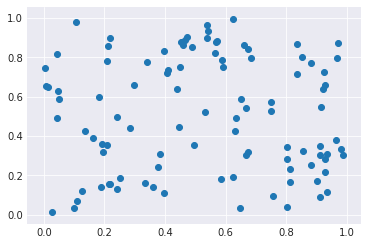
\includegraphics[height=0.50\textheight]{fig/scatterplot.pdf}
%   \end{center}
% \end{frame}


% \begin{frame}[fragile]
%   \frametitle{Bar plots}

%   Use Seaborn's \texttt{sea.barplot(x, y)} function.

%   \+
%   Everything else works \emph{almost} as in line plots; when you need to plot
%   onto an axis (the \texttt{ax} object of previous examples), then you need to
%   pass the axis as an additional parameter:
% \begin{semiverbatim}
% sea.barplot(x, y, ax=ax)
% \end{semiverbatim}
% \end{frame}


\part{Appendix}

\subsection{Collections}

%%% set container

\begin{frame}[fragile]
  \frametitle{Sets (1)} The \texttt{set} type implements an
  \textbf{unordered} container that holds exactly one object per
  equivalence class:
\begin{lstlisting}
>>> S = set()
>>> S.add(1)
>>> S.add('two')
>>> S.add(1)
>>> S
set([1, 'two'])
\end{lstlisting}

\end{frame}


\begin{frame}[fragile]
  \frametitle{Sets (2)}
You can create a set and add elements to it in one go:
\begin{lstlisting}
>>> S2 = set([1, 2, 3, 4])
\end{lstlisting}

and remove elements:

\begin{lstlisting}
>>> S2.remove(2)
>>> S2.pop()
1
>>> S2
set([3,4])
\end{lstlisting}
\end{frame}


\begin{frame}[fragile]
  \frametitle{Sets (3)}
  Sets are often used to get unique values from a list:
  \begin{lstlisting}
>>> L = [1, 1, 2, 2, 3, 3]
>>> set(L)
set([1, 2, 3])
 \end{lstlisting}

\+\pause
Of course, you can also create a list from a set:
\begin{lstlisting}
>>> S = set((1,2,3))
>>> list(S)
[1, 2, 3]
\end{lstlisting}

\+\pause
\begin{question}
  In what order will the set items appear \\ in the resulting list?
\end{question}

\end{frame}

%%% tuples

\begin{frame}[fragile]
  \frametitle{Tuples}
  Tuples are like lists
  \begin{lstlisting}
>>> T = (1, 2, 3)
>>> T[0]
1
>>> T[0:1]
(1,)
  \end{lstlisting}

  \+
but they are \textit{immutable}

\begin{lstlisting}[basicstyle=\footnotesize\ttfamily]
>>> T[0] = 'a'
Traceback (most recent call last):
  File "<stdin>", line 1, in <module>
TypeError: 'tuple' object does not support item assignment
\end{lstlisting}
\end{frame}

% %%% multiple assignment

\begin{frame}[fragile]
\frametitle{Multiple assignment}
% aka "destructuring bind"
You can assing multiple variables at the same time
\begin{lstlisting}
>>> a, b, c = (1, 2, 3)
>>> print(a)
1
>>> print(b)
2
\end{lstlisting}

\+

It works with any sequence:

\begin{lstlisting}
>>> a, b, c = 'UZH'
>>> print(a)
U
\end{lstlisting}

\pause
\begin{question}
  Can you think of a way to swap the values of two variables using this?
\pause
\begin{lstlisting}
>>> a, b = b, a
\end{lstlisting}
\end{question}
\end{frame}

\begin{frame}[fragile]
\frametitle{Multiple assignment (2)}
Multiple assignment can be used in \texttt{for} statements as well.
\begin{lstlisting}
>>> L = [(1,'a'), (2,'b'), (3, 'c')]
>>> for x, y in L:
...     print ("first is " + str(x)
...            + ' and second is ' + y)
\end{lstlisting}

  \+
  This is particularly useful with functions that return a tuple.
  For instance the \texttt{enumerate()} function (look it up with
  \texttt{help()}!).
\end{frame}


%%% data structures recap

\begin{frame}
  \frametitle{Data structures recap}
  \begin{center}
    \begin{tabular}{>{\ttfamily}c|>{\ttfamily}c|>{\footnotesize}p{0.5\linewidth}}
      \rmfamily \textbf{mutable} & \rmfamily \textbf{immutable} & \\
      set & frozenset & unordered container of
      unique elements\\[1ex]
      list & tuple & ordered sequence\\[1ex]
      dict & $-$ & key/values mapping\\[1ex]
      $-$& str & ordered sequence of characters\\
    \end{tabular}
  \end{center}
\end{frame}


% \begin{frame}[fragile]
%   \frametitle{Useful data structures operations}

%   Read {\url{http://docs.python.org/tutorial/datastructures.html}}.

%   \+
%   Really, you will need it.

%   \+
%   And remember that \texttt{dir()} and \texttt{help()} are your friends!
% \end{frame}


\end{document}

%%% Local Variables:
%%% mode: latex
%%% TeX-master: t
%%% End:
